% =============================================
% CAPÍTULO 1 - CONTEXTUALIZAÇÃO
% =============================================
\chapter{CONTEXTUALIZAÇÃO}

A transformação digital no setor financeiro ampliou as possibilidades de acesso e uso de dados pelos usuários. Nesse contexto, o \textit{Open Finance} se destaca por permitir o compartilhamento padronizado de informações financeiras entre instituições autorizadas, mediante consentimento do cliente, favorecendo o desenvolvimento de soluções mais integradas e personalizadas (BANCO CENTRAL DO BRASIL; CONSELHO MONETÁRIO NACIONAL, 2020). Ao mesmo tempo, a expansão desse ecossistema no Brasil e a ampla presença de canais de comunicação digital no cotidiano das pessoas reforçam a oportunidade de criação de serviços financeiros mais acessíveis, próximos e orientados pela rotina do usuário (BANCO CENTRAL DO BRASIL, 2025; META PLATFORMS, INC., [s. d.]).

Apesar desses avanços, a gestão financeira pessoal ainda apresenta limitações, pois muitas soluções permanecem centradas em \textit{dashboards}, extratos e gráficos em aplicativos ou plataformas \textit{web}, exigindo consultas ativas e pouco integradas ao dia a dia. Além disso, o baixo nível de letramento financeiro digital observado em estudos internacionais realizados pela \textit{Organisation for Economic Co-operation and Development} reforça a necessidade de soluções que simplifiquem a interpretação das informações financeiras (OECD, 2023).

Diante disso, este trabalho propõe o desenvolvimento de uma solução de assistência financeira inteligente operada integralmente por meio do WhatsApp, integrando dados obtidos via \textit{Open Finance} a técnicas de análise preditiva e a um assistente conversacional baseado em \textit{Retrieval-Augmented Generation}, a fim de oferecer consultas, alertas e recomendações personalizadas em linguagem natural. A proposta justifica-se pela busca de maior acessibilidade, usabilidade e apoio contínuo à tomada de decisão, sem dependência de uma plataforma \textit{web} tradicional, observando também requisitos de privacidade e proteção de dados previstos na LGPD.

\section{Objetivo}

Desenvolver uma solução de assistência financeira inteligente, operada integralmente por meio do WhatsApp, capaz de integrar dados do \textit{Open Finance} e fornecer ao usuário análises, previsões e orientações personalizadas para apoiar a tomada de decisões financeiras.

\section{Público-alvo}

O público-alvo do negócio é formado, principalmente, por adultos economicamente ativos que já utilizam serviços bancários digitais e buscam maior controle sobre sua vida financeira de forma simples, prática e acessível. Enquadram-se nesse perfil estudantes, trabalhadores assalariados, autônomos, microempreendedores e demais usuários que têm dificuldade e desejam acompanhar gastos, organizar orçamento, prever compromissos financeiros e transformar dados bancários em decisões do dia a dia. As estratégias do negócio devem ser direcionadas a pessoas que já usam o WhatsApp como canal recorrente de comunicação, aproveitando o fato de que a plataforma permite interações empresariais em escala por meio da \textit{WhatsApp Business Platform} e se encaixa na rotina cotidiana do usuário, reduzindo barreiras de adoção tecnológica. Além disso, como a proposta depende da integração com dados financeiros compartilhados mediante consentimento no ecossistema de \textit{Open Finance}, o serviço tende a ser especialmente relevante para usuários que desejam centralizar informações bancárias e receber orientações personalizadas em linguagem natural, sem precisar acessar uma plataforma \textit{web} tradicional.

\subsection{Personas}

As personas consistem em perfis fictícios elaborados com base nas características, comportamentos, necessidades e dificuldades do público que se pretende atender. Sua utilização no projeto permite compreender com maior profundidade os diferentes tipos de usuários, suas expectativas em relação à solução proposta e a forma como interagem com tecnologias voltadas à organização financeira. A partir dessa construção, torna-se possível orientar decisões de desenvolvimento com maior foco na experiência do usuário, na usabilidade e na adequação das funcionalidades ao contexto real de uso. Neste trabalho, foram definidas três personas que representam perfis contrastantes, mas ambos compatíveis com o público-alvo da solução, conforme apresentado nas Figuras X, X e X.

\begin{figure}[H]
    \centering
    \caption{Esquema de uma infraestrutura de \textit{Botnet}.}
    \label{fig:botnet}
    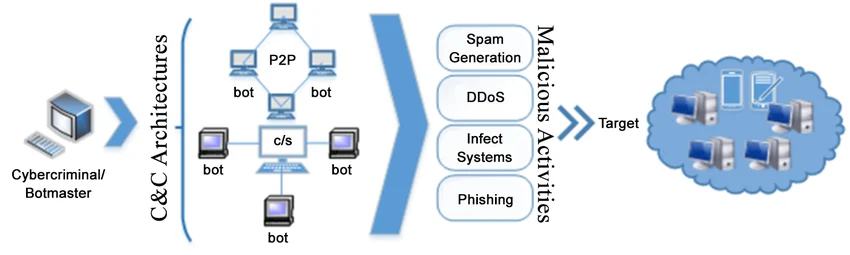
\includegraphics[width=1\textwidth]{images/botnet.png}
\end{figure}
{\setstretch{1.0}\fontetabela{\textbf{Fonte:} Elaborado pelos autores (2026).}}

% Figura X: Persona 2
% Fonte: elaborado pelos autores (2026)

% Figura X: Persona 3
% Fonte: elaborado pelos autores (2026)

\section{Conceito do produto}

O produto proposto consiste em uma solução de assistência financeira inteligente operada integralmente por meio do WhatsApp, voltada a usuários que desejam acompanhar melhor sua vida financeira sem depender de uma plataforma \textit{web} tradicional. Sua principal finalidade é atender necessidades como organização do orçamento, compreensão dos hábitos de consumo, acompanhamento do histórico bancário, identificação de padrões de gastos e apoio à tomada de decisão financeira no cotidiano. Para isso, a solução utiliza dados compartilhados pelo usuário no ecossistema de \textit{Open Finance}, que prevê o compartilhamento padronizado de informações mediante autorização do cliente e em ambiente seguro, e integra esses dados a uma interface conversacional mais simples e próxima da rotina do público-alvo.

Como diferencial, o produto busca unir três elementos centrais em uma única experiência: a centralização de dados financeiros, a análise preditiva personalizada e a interação em linguagem natural dentro de um canal já amplamente utilizado pelos usuários. Em vez de exigir acesso recorrente a \textit{dashboards} e telas específicas, a proposta desloca a experiência para o WhatsApp, plataforma que permite comunicação estruturada entre empresas e clientes em escala. Assim, o sistema pretende oferecer respostas, alertas e recomendações de maneira mais acessível, prática e contextualizada, reduzindo barreiras de uso e aumentando a proximidade com o usuário.

Entre os principais riscos do produto, destacam-se a dependência do consentimento do usuário e da disponibilidade das integrações com instituições participantes do \textit{Open Finance}, os desafios relacionados à privacidade e à proteção de dados financeiros, e a necessidade de garantir interpretações confiáveis por parte da inteligência artificial, evitando respostas imprecisas ou excessivamente genéricas. Além disso, por operar no WhatsApp, a solução também depende do cumprimento das políticas da plataforma, que prevê mecanismos de fiscalização e restrições para contas empresariais que violem suas regras de uso. Dessa forma, o sucesso do produto depende não apenas da qualidade técnica da solução, mas também da conformidade regulatória, da segurança da informação e da construção de confiança na interação com o usuário.
